\chapter{Los microbios y la infección}\label{ch:g9:microbes-and-infection}

Vienen siguiendo a este libro desde los gérmenes invisibles de primero
(\cref{def:g1:healthy-habits:germs}): ascendidos a plantilla en la
panadería (\cref{ch:g6:producing-our-food}), a cuadrillas de
\omterm{def:g6:decomposers-and-soil:decomposers}{descomponedores} en el \omterm{def:g6:decomposers-and-soil:soil}{suelo} y a adversario que evoluciona en la sala
del hospital (\cref{ex:g9:how-species-change:resistance}). Este
capítulo por fin les rinde cuentas enteras a los \omterm{def:g6:producing-our-food:fermentation}{microbios}: qué son,
cómo ataca la minoría dañina y cómo aguantan las puertas las defensas
exteriores del cuerpo --- y las nuestras.

\section{El mundo microbiano}

\begin{definition}[Los microbios, ordenados]\label{def:g9:microbes-and-infection:sorted}
Los \emph{microorganismos}\index{microorganismo} --- los \omterm{def:g6:producing-our-food:fermentation}{microbios} ---
son \omterm{def:g6:exploring-our-environment:components}{seres vivos} demasiado pequeños para verlos a simple vista. Las
clases principales:
\begin{itemize}
  \item las \emph{bacterias}\index{bacteria}: \omterm{def:g5:first-look-at-cells:cell}{células} sueltas sin
        \omterm{def:g6:cell-unit-of-life:parts}{núcleo} verdadero, muchísimo más pequeñas que las tuyas, que se
        dividen deprisa (el mundo de la
        \cref{def:g6:cell-unit-of-life:unicellular}) --- por todas
        partes y en números que no se pueden contar;
  \item los \emph{\omterm{def:g6:decomposers-and-soil:decomposers}{hongos} y otros seres de una sola \omterm{def:g5:first-look-at-cells:cell}{célula}}: las
        \omterm{ex:g6:producing-our-food:bread}{levaduras} (\cref{ex:g6:producing-our-food:bread}), las \omterm{def:g4:plants-without-seeds:spore}{esporas}
        de los mohos, los nadadores de la gota de estanque;
  \item los \emph{virus}\index{virus}: más pequeños todavía y
        distintos por su clase --- un retal de texto genético
        empaquetado (las letras de la
        \cref{def:g9:genes-and-dna:dna}) dentro de una cubierta, y
        \emph{sin \omterm{def:g5:first-look-at-cells:cell}{célula} y sin vida propia}: un virus no hace nada
        hasta que entra en una \omterm{def:g5:first-look-at-cells:cell}{célula} viva y pone la maquinaria de
        lectura de esa \omterm{def:g5:first-look-at-cells:cell}{célula} a copiar el texto del intruso. En las
        señales de la \cref{prop:g1:living-or-not:signs}, los virus
        están justo en el borde de la vida.
\end{itemize}
\end{definition}

\begin{proposition}[Casi todos inofensivos, muchos imprescindibles]\label{prop:g9:microbes-and-infection:mostly}
La fama de dañinos es el informe de una minoría. Casi todos los
\omterm{def:g6:producing-our-food:fermentation}{microbios} nos ignoran, y muchos nos sirven: las cuadrillas de
\omterm{def:g6:decomposers-and-soil:decomposers}{descomponedores} (\cref{def:g6:decomposers-and-soil:decomposers}), las
plantillas de la alimentación, los químicos del \omterm{def:g6:decomposers-and-soil:soil}{suelo} --- y tu propia
\emph{flora residente}\index{flora residente}: los billones de
\omterm{def:g9:microbes-and-infection:sorted}{bacterias} inofensivas que alfombran la \omterm{def:g1:the-five-senses:sense}{piel} y el intestino, ayudan a la
\omterm{def:g4:journey-of-food:digestion}{digestión} y, por pura ocupación, les quitan el sitio a los intrusos.
Solo una pequeña minoría --- los \emph{patógenos}\index{patógeno} ---
causa enfermedades.
\end{proposition}
\admitted

\begin{example}[Un cuerpo, tres relaciones]\label{ex:g9:microbes-and-infection:relations}
En tu \omterm{def:g1:the-five-senses:sense}{piel} en este momento: residentes a miles de millones, aguantando
la superficie (relación uno: alianza). En tu yogur del desayuno:
trabajadores, agriando por encargo (relación dos: empleo,
\cref{ex:g6:producing-our-food:yogurt}). En el clavo oxidado del
cobertizo: \omterm{def:g4:plants-without-seeds:spore}{esporas} de la \omterm{def:g9:microbes-and-infection:sorted}{bacteria} del tétanos, esperando un corte hondo
(relación tres: la minoría patógena y la razón del
\cref{ch:g9:immune-defenses} y de la dosis de recuerdo del tétanos).
\end{example}

\section{La infección: el ataque, por etapas}

\begin{definition}[Las etapas de la infección]\label{def:g9:microbes-and-infection:stages}
La \emph{infección}\index{infección} corre por etapas, cada una con su
nombre:
\begin{enumerate}
  \item la \emph{transmisión}: el patógeno viaja --- superficies
        tocadas y manos, gotitas de tos, comida y agua contaminadas,
        \omterm{prop:g4:journey-of-food:absorb}{sangre} y la vía sexual que señaló la
        \cref{def:g8:contraception:condom};
  \item la \emph{entrada}: por una brecha --- la \omterm{def:g1:the-five-senses:sense}{piel} cortada --- o por
        las puertas abiertas del cuerpo: las vías respiratorias, el
        \omterm{def:g4:journey-of-food:tract}{tubo digestivo} y las vías de arriba;
  \item la \emph{multiplicación}: calientes, húmedos y alimentados, los
        recién llegados se dividen --- las \omterm{def:g9:microbes-and-infection:sorted}{bacterias} por la regla de
        las \omterm{def:g6:exploring-our-environment:conditions}{condiciones} de la
        \cref{prop:g6:decomposers-and-soil:speed}, doblando su número
        cada pocas horas; los \omterm{def:g9:microbes-and-infection:sorted}{virus} convirtiendo \omterm{def:g5:first-look-at-cells:cell}{células} en
        copisterías;
  \item la \emph{enfermedad}: los síntomas --- del daño mismo, de los
        venenos bacterianos y en parte (capítulo siguiente) de la
        propia batalla de la defensa.
\end{enumerate}
\end{definition}

\begin{example}[Dos invasores, contrastados]\label{ex:g9:microbes-and-infection:contrast}
La \omterm{def:g9:microbes-and-infection:sorted}{bacteria} del corte contra el \omterm{def:g9:microbes-and-infection:sorted}{virus} del catarro de invierno. La
\omterm{def:g9:microbes-and-infection:sorted}{bacteria}: entra por la brecha, se multiplica \emph{entre} las \omterm{def:g5:first-look-at-cells:cell}{células}
del tejido caliente y húmedo, y sus desechos envenenan el vecindario
--- el \omterm{def:g4:heart-and-blood:heart}{latido} y el pus de un dedo infectado. El \omterm{def:g9:microbes-and-infection:sorted}{virus}: viaja en una
gotita hasta el revestimiento de las vías respiratorias, entra en las
\omterm{def:g5:first-look-at-cells:cell}{células} mismas de ese revestimiento, y cada \omterm{def:g5:first-look-at-cells:cell}{célula} secuestrada suelta
una multitud de copias antes de fallar --- la garganta en carne viva y
la nariz que chorrea de su rastro. Mecánicas distintas; el antibiótico
que mata de hambre a la primera no puede tocar al segundo, porque el
segundo toma prestada \emph{tu} maquinaria y los medicamentos contra él
son difíciles de apuntar.
\end{example}

\section{Aguantar las puertas}

\begin{proposition}[Las primeras defensas]\label{prop:g9:microbes-and-infection:doors}
Antes de cualquier batalla, el cuerpo aguanta sus fronteras:
\begin{itemize}
  \item la \emph{\omterm{def:g1:the-five-senses:sense}{piel}}: seca, en capas y que se renueva sola --- la
        muralla (el órgano de la
        \cref{def:g1:the-five-senses:sense}, de guarnición);
  \item los \emph{revestimientos y sus escobas}: las superficies de
        limpieza de las vías respiratorias
        (\cref{prop:g7:lungs-and-gas-exchange:smoke} las enseñó
        desbordadas), la química de aclarado de las lágrimas y la
        \omterm{def:g4:journey-of-food:tract}{saliva}, y el baño de ácido del \omterm{def:g4:journey-of-food:tract}{estómago}
        (\cref{pb:g7:digestion-and-nutrients:1} esteriliza mientras
        digiere);
  \item los \emph{residentes}: el terreno ocupado por la flora, con
        poco sitio para desembarcos;
\end{itemize}
y la \omterm{def:g1:healthy-habits:hygiene}{higiene} las alarga: el jabón del
\cref{met:g1:healthy-habits:hands} (ahora con su mecanismo entero ---
la transmisión interrumpida), el agua potable, la comida cocinada y
guardada en frío (la negativa de \omterm{def:g6:exploring-our-environment:conditions}{condiciones} de la
\cref{rem:g6:producing-our-food:goodbad}), la aguja esterilizada, la
barrera del \omterm{def:g8:contraception:condom}{preservativo}. Todas las reglas de \omterm{def:g1:healthy-habits:hygiene}{higiene} de este libro son
una etapa de transmisión o de entrada, bloqueada.
\end{proposition}
\admitted

\begin{omfigure}
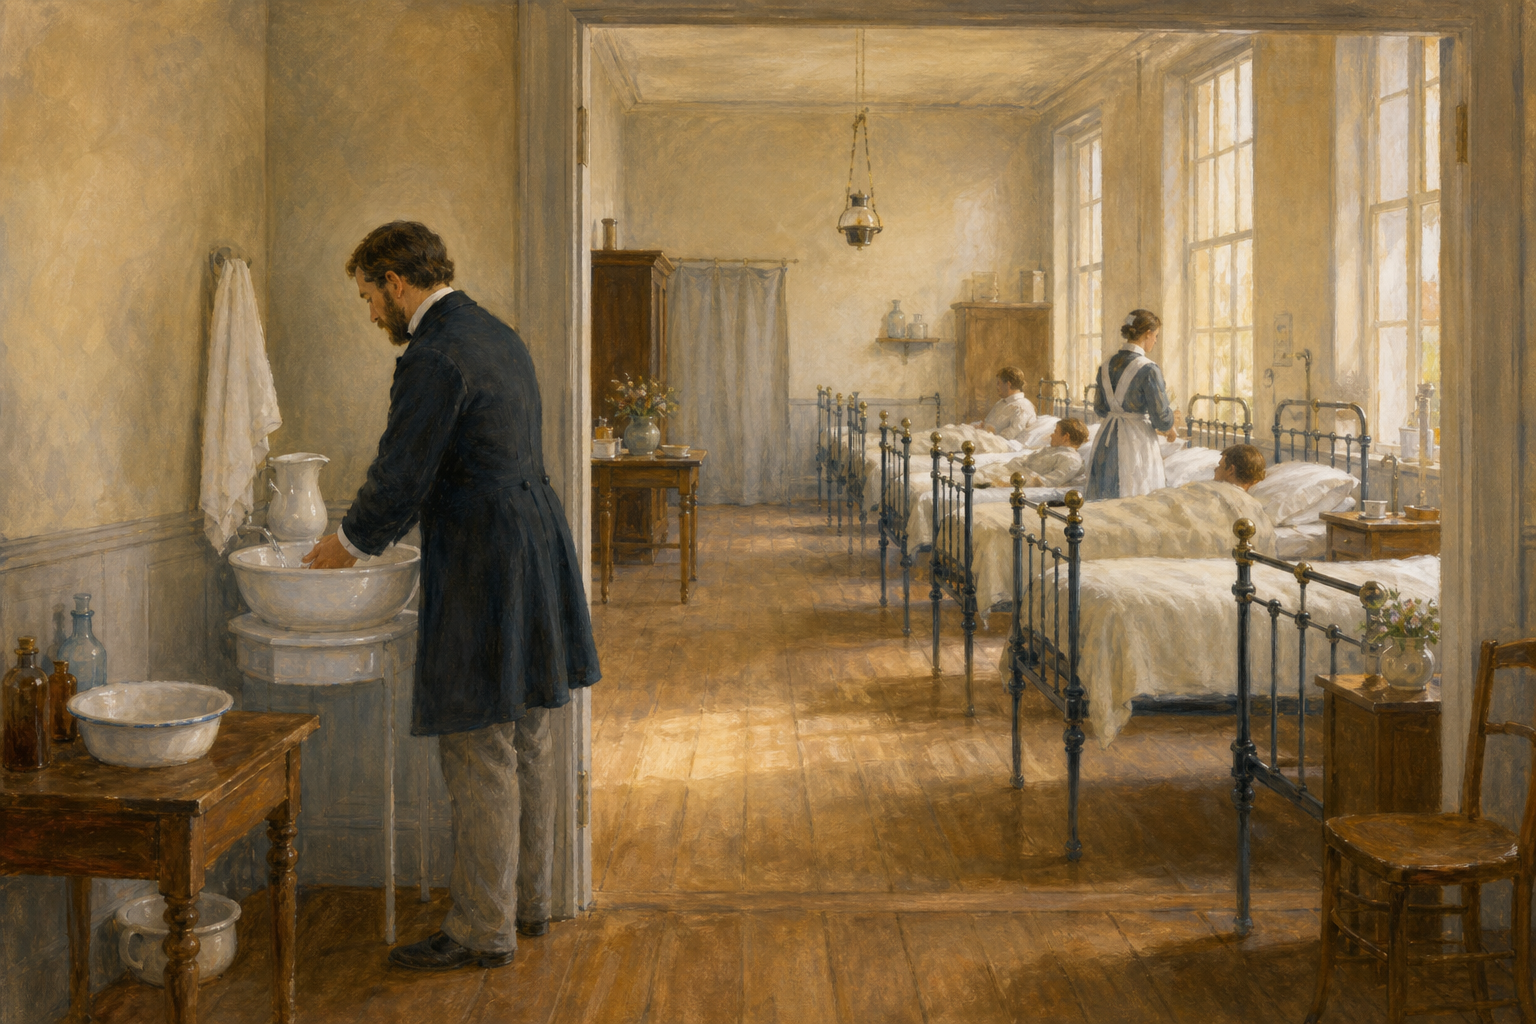
\includegraphics[width=0.6\linewidth]{images/book1/ai/g9-microbe-washing.png}

{\small La medicina más barata de la historia: una palangana en la
puerta de la sala, interrumpiendo a unos mensajeros que no ve ningún \omterm{def:g1:the-five-senses:sense}{ojo}.}
\end{omfigure}

\begin{example}[Los dos médicos que movieron los números]\label{ex:g9:microbes-and-infection:history}
Dos nombres anclan la historia. Semmelweis, en la Viena de los años
cuarenta del siglo XIX: las muertes por fiebre puerperal se desplomaron
en su sala de maternidad cuando los médicos se lavaron las manos entre
la sala de autopsias y el parto --- transmisión interrumpida antes de
que nadie hubiera visto al viajero. Pasteur, una generación después,
enseñó a los viajeros mismos: \omterm{def:g6:producing-our-food:fermentation}{microbios}, y no ``aire malo'', agriando
el vino, matando a los gusanos de seda e infectando las heridas --- y
el calor (su \emph{pasteurización}) o la esterilización parándolos. La
teoría de los gérmenes convirtió los hospitales de peligros en defensas
en el espacio de una vida.
\end{example}

\begin{omfigure}
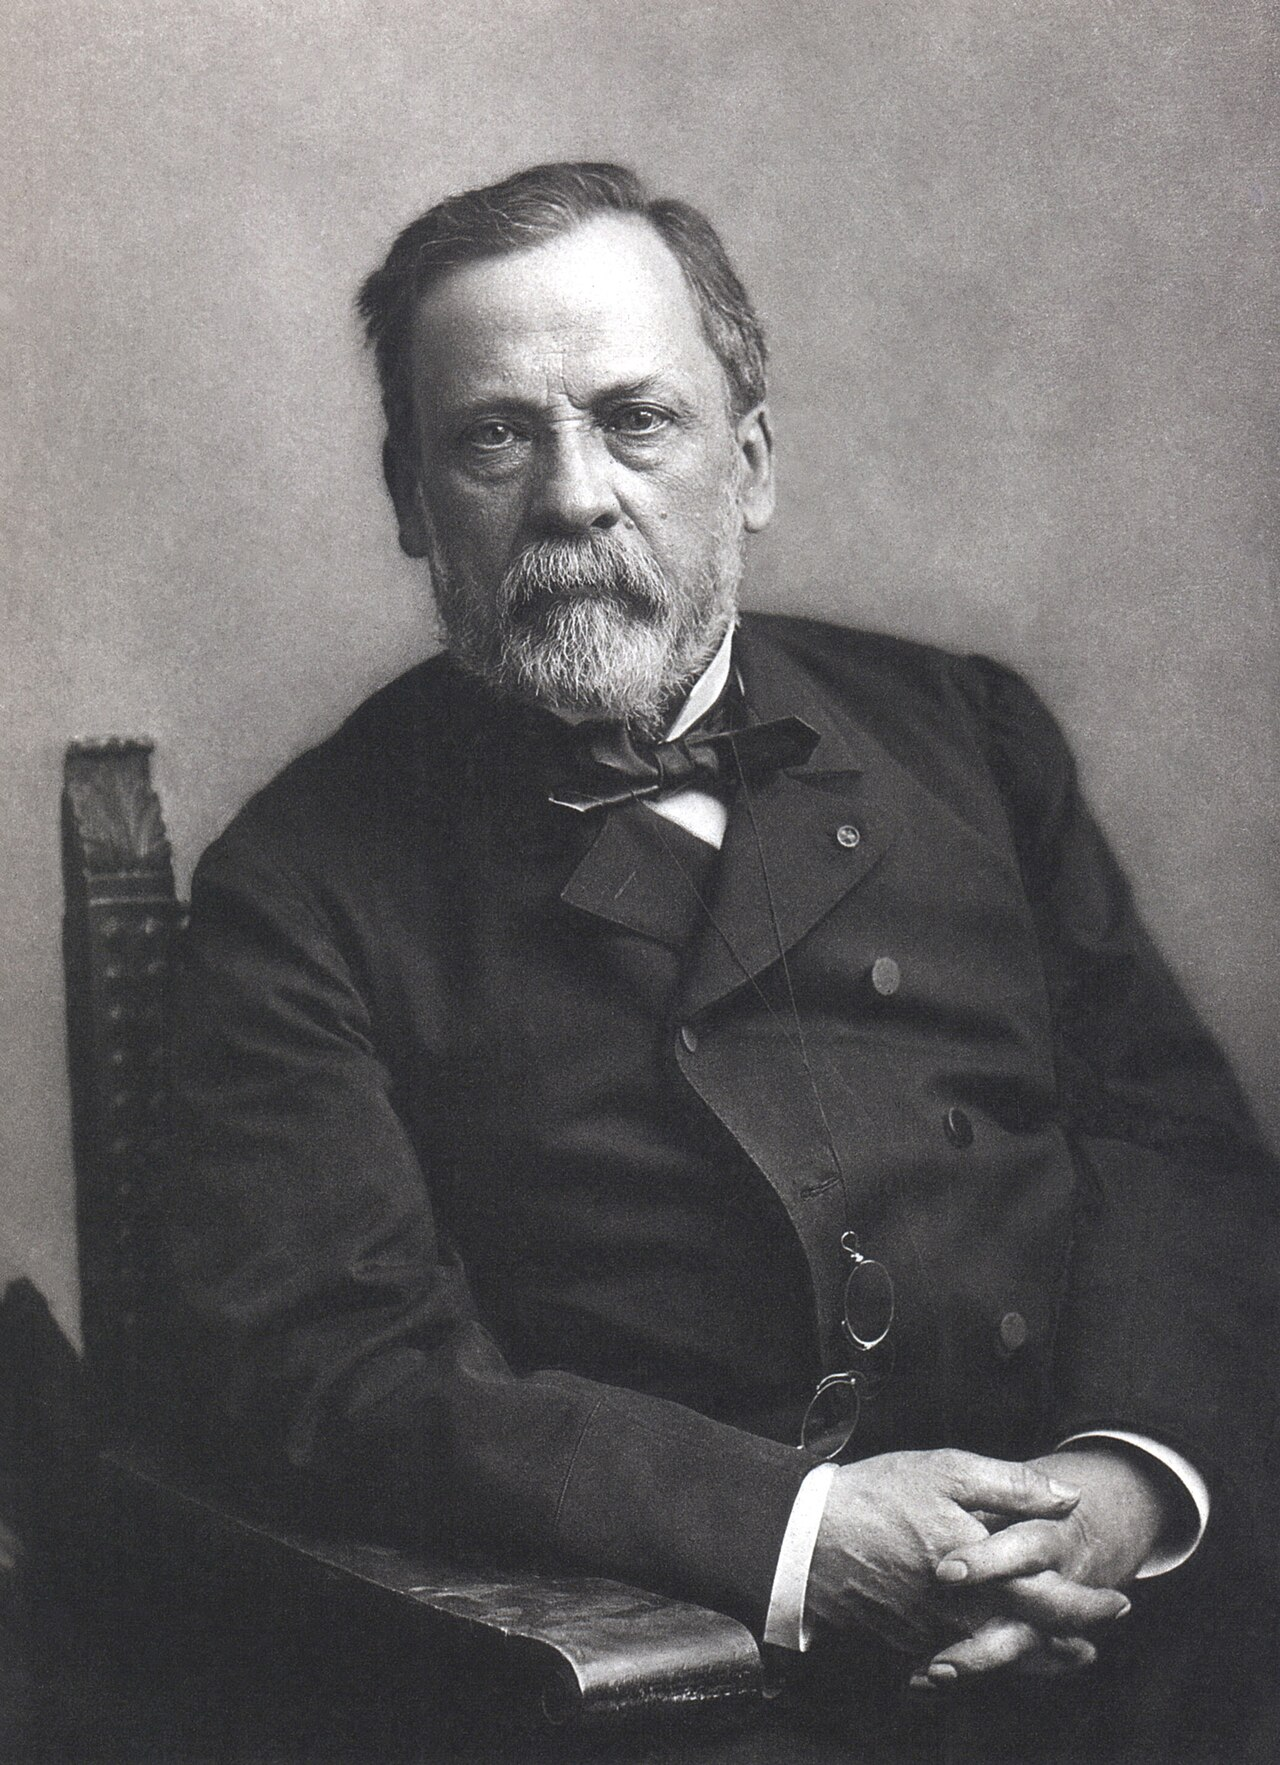
\includegraphics[width=0.42\linewidth]{images/book1/pasteur.jpg}

{\small Louis Pasteur, fotografiado por Paul Nadar: el científico que
enseñó a los viajeros invisibles en persona.}
\end{omfigure}

\begin{method}[Auditar un riesgo de infección]\label{met:g9:microbes-and-infection:audit}
Para cualquier situación --- cocina, herida, sala de hospital, multitud:
\begin{enumerate}
  \item nombra el patógeno verosímil y su clase (\omterm{def:g9:microbes-and-infection:sorted}{bacteria}, \omterm{def:g9:microbes-and-infection:sorted}{virus},
        \omterm{def:g6:decomposers-and-soil:decomposers}{hongo});
  \item sigue su vía de transmisión hasta ti;
  \item encuentra su puerta de entrada;
  \item pregunta qué lo multiplica --- calor, \omterm{def:g6:exploring-our-environment:conditions}{humedad}, comida, tiempo;
  \item bloquea la etapa más barata: lavar, cocinar, cubrir, enfriar,
        esterilizar, vacunar (el \cref{ch:g9:immune-defenses} explica
        lo último).
\end{enumerate}
\end{method}

\section{Ejercicios}

\begin{exercise}[$\star$]\label{exo:g9:microbes-and-infection:1}
Nombra las clases principales de \omterm{def:g1:healthy-habits:germs}{microbio} y qué distingue a los \omterm{def:g9:microbes-and-infection:sorted}{virus}.
\end{exercise}

\begin{exercise}[$\star$]\label{exo:g9:microbes-and-infection:2}
¿Qué es la \omterm{prop:g9:microbes-and-infection:mostly}{flora residente} y qué dos servicios presta?
\end{exercise}

\begin{exercise}[$\star$]\label{exo:g9:microbes-and-infection:3}
Enumera las cuatro etapas de la \omterm{def:g9:microbes-and-infection:stages}{infección} con un ejemplo de cada una.
\end{exercise}

\begin{exercise}[$\star$]\label{exo:g9:microbes-and-infection:4}
Contrasta el corte infectado y el catarro: ¿dónde se multiplica cada
invasor?
\end{exercise}

\begin{exercise}[$\star$]\label{exo:g9:microbes-and-infection:5}
Nombra cuatro primeras defensas y la etapa que aguanta cada una.
\end{exercise}

\begin{exercise}[$\star$]\label{exo:g9:microbes-and-infection:6}
¿Qué interrumpió el lavado de manos de Semmelweis, y qué añadió
Pasteur?
\end{exercise}

\begin{exercise}[$\star\star$]\label{exo:g9:microbes-and-infection:7}
¿Por qué dejan intactos los antibióticos a los catarros? Responde con
las mecánicas de los dos invasores.
\end{exercise}

\begin{exercise}[$\star\star$]\label{exo:g9:microbes-and-infection:8}
Vuelve a deducir tres reglas de \omterm{def:g1:healthy-habits:hygiene}{higiene} de la infancia
(\cref{ch:g1:healthy-habits}) como bloqueos de etapa, nombrando el
mecanismo.
\end{exercise}

\begin{exercise}[$\star\star$]\label{exo:g9:microbes-and-infection:9}
Pasa el \cref{met:g9:microbes-and-infection:audit} por la ensalada de
pollo de un picnic de verano, calentada tres horas en un coche.
\end{exercise}

\begin{exercise}[$\star\star$]\label{exo:g9:microbes-and-infection:10}
¿Por qué importa más lavarse las manos \emph{entre} tareas que
lavárselas a menudo? (La sala de Semmelweis tiene la respuesta.)
\end{exercise}

\begin{exercise}[$\star\star$]\label{exo:g9:microbes-and-infection:11}
Sitúa la sala de hospital del
\cref{ex:g9:how-species-change:resistance} en este capítulo: ¿qué etapa
ataca el antibiótico, y qué cría su uso a medias?
\end{exercise}

\begin{exercise}[$\star\star\star$]\label{exo:g9:microbes-and-infection:12}
``Un \omterm{def:g9:microbes-and-infection:sorted}{virus} es un texto que toma prestada una impresora''. Despliega la
imagen con la \cref{def:g9:genes-and-dna:dna} y la
\cref{def:g9:microbes-and-infection:sorted} --- y úsala para decir por
qué están los \omterm{def:g9:microbes-and-infection:sorted}{virus} en el borde de la vida y por qué es difícil
atacarlos con medicamentos.
\end{exercise}

\section{Problema: El cuaderno del brote}

\begin{problem}[{Problema de fin de semana --- un brote escolar,
seguido etapa a etapa}]\label{pb:g9:microbes-and-infection:1}
Un brote escolar (de ficción): en una semana, la mitad de la clase de
9.º B declara fiebre y tos; después van saliendo casos sueltos en las
demás clases. La enfermera del colegio lleva un cuaderno del brote y le
pide a la clase de \omterm{def:g1:living-or-not:living}{biología} que la ayude a leerlo.

\medskip\noindent\textbf{Parte I --- Leer la propagación.}
\begin{enumerate}
  \item El primer caso --- el índice --- se sentaba en 9.º B; los ocho
        siguientes comparten su fila y sus parejas de tenis de mesa.
        Nombra la vía de transmisión probable y la puerta de entrada.
  \item Los casos se doblan cada dos días al principio. ¿La aritmética
        de qué etapa se está viendo, y de quién es la maquinaria que
        está haciendo las copias si el agente es un \omterm{def:g9:microbes-and-infection:sorted}{virus}?
  \item La lista de la enfermera: comienzo de la fiebre, tos, garganta
        en carne viva. ¿Qué etapa marcan los síntomas, y de qué dos
        fuentes surgen?
  \item ¿Por qué saltó el brote de clase en clase justamente en las dos
        asambleas de todo el colegio de esa semana?
\end{enumerate}

\medskip\noindent\textbf{Parte II --- El contraataque.}
\begin{enumerate}[resume]
  \item Las medidas del colegio: los alumnos enfermos a casa; las
        ventanas abiertas (\cref{exo:g4:breathing:10}); el lavado de
        manos ensayado; el material compartido limpiado. Asígnale a
        cada medida la etapa que bloquea.
  \item Un padre exige antibióticos para todos. Redacta la respuesta
        del médico para un brote vírico --- y la advertencia sobre la
        selección (\cref{exo:g9:how-species-change:10}) si se
        esparcieran antibióticos de todos modos.
  \item El comedor declara a la vez dos casos de \omterm{def:g4:journey-of-food:tract}{estómago} que se siguen
        hasta un postre sin refrigerar. Audita ese brote lateral con el
        \cref{met:g9:microbes-and-infection:audit} --- otra clase de
        agente, otras etapas.
  \item ¿Por qué dibuja la enfermera un mapa de \emph{quién se sentaba
        dónde} en lugar de tratar los casos como si fueran al azar?
        ¿Qué es un mapa de brote, en términos de transmisión?
\end{enumerate}

\medskip\noindent\textbf{Parte III --- El balance.}
\begin{enumerate}[resume]
  \item Escribe la biografía del brote en las cuatro etapas, del caso
        índice hasta que se apaga.
  \item El brote se apagó antes de llegar a todos los alumnos. Ofrece
        dos mecanismos --- los bloqueos de las medidas y la pista del
        capítulo siguiente: los que ya eran inmunes por la cepa prima
        del año pasado.
  \item Añade el párrafo de historia: ¿de qué dos lecciones del siglo
        XIX (\cref{ex:g9:microbes-and-infection:history}) descendía la
        respuesta entera del colegio?
  \item Cierra el cuaderno con el método de auditoría convertido en
        lema: una frase sobre dónde sale más barato parar los brotes.
\end{enumerate}
\end{problem}
